   \begin{figure}[h]
        \centering
		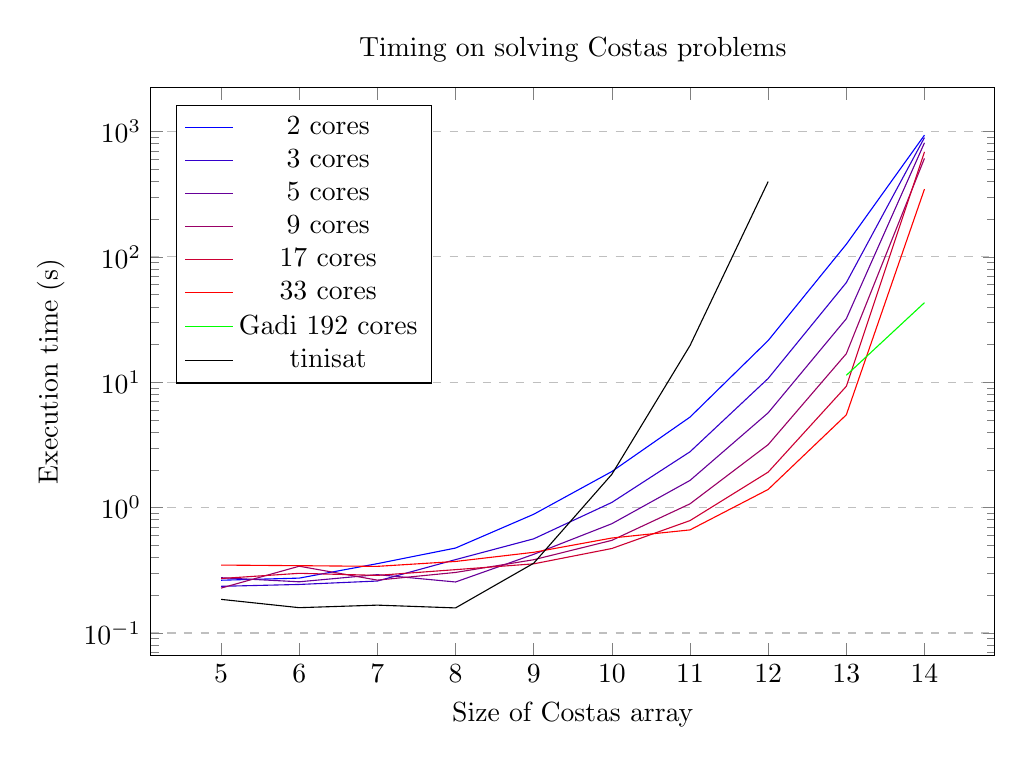
\begin{tikzpicture}
		\begin{axis}[
			title={Timing on solving Costas problems},
			xlabel={Size of Costas array},
			ylabel={Execution time (s)},
			%xmin=0, xmax=0.25,
			%ymin=10.00, ymax=100000.00,
			ymode=log,
			%xmode=log,
			%xtick={0,0.05,0.1,0.15,0.2,0.25},
			%ytick={0,20,40,60,80,100},
			%yticklabel=$\pgfmathprintnumber{\tick}\%$,
			legend pos=north west,
			ymajorgrids=true,
			grid style=dashed,
			xticklabel style={/pgf/number format/fixed},
			width = 350,
			height = 250
		]


\addplot[color=red!0.0!blue,line width=0.4pt] coordinates {
(5,0.263445615768433)(6,0.27386999130249)(7,0.357252597808838)(8,0.475878000259399)(9,0.884846210479736)(10,1.94017291069031)(11,5.27208352088928)(12,21.5157859325409)(13,126.130258560181)(14,935.905344486237)
}node[pos=0.8](endofplotsquare){} ;
\addlegendentry{2 cores}
\addplot[color=red!20.0!blue,line width=0.4pt] coordinates {
(5,0.235576391220093)(6,0.243774652481079)(7,0.259596824645996)(8,0.384731769561768)(9,0.563618898391724)(10,1.09974837303162)(11,2.78815150260925)(12,10.7241916656494)(13,62.3517887592316)(14,894.68763256073)
}node[pos=0.8](endofplotsquare){} ;
\addlegendentry{3 cores}
\addplot[color=red!40.0!blue,line width=0.4pt] coordinates {
(5,0.275908231735229)(6,0.255989551544189)(7,0.291936635971069)(8,0.25504994392395)(9,0.423865795135498)(10,0.7440185546875)(11,1.64754581451416)(12,5.70390057563782)(13,32.111976146698)(14,813.767755270004)
}node[pos=0.8](endofplotsquare){} ;
\addlegendentry{5 cores}
\addplot[color=red!60.0!blue,line width=0.4pt] coordinates {
(5,0.227974414825439)(6,0.340758323669434)(7,0.263911247253418)(8,0.303909063339233)(9,0.383917570114136)(10,0.547943830490112)(11,1.0718412399292)(12,3.17991042137146)(13,16.8961277008057)(14,610.471871614456)
}node[pos=0.8](endofplotsquare){} ;
\addlegendentry{9 cores}
\addplot[color=red!80.0!blue,line width=0.4pt] coordinates {
(5,0.271912097930908)(6,0.299091815948486)(7,0.287986755371094)(8,0.319964408874512)(9,0.355975151062012)(10,0.471837759017944)(11,0.787814617156982)(12,1.91974759101868)(13,9.27965927124023)(14,688.911826848984)
}node[pos=0.8](endofplotsquare){} ;
\addlegendentry{17 cores}
\addplot[color=red!100.0!blue,line width=0.4pt] coordinates {
(5,0.34800124168396)(6,0.344078302383423)(7,0.339888334274292)(8,0.371899843215942)(9,0.439922332763672)(10,0.571996927261353)(11,0.663976430892944)(12,1.39575672149658)(13,5.49585580825806)(14,347.331707239151)
}node[pos=0.8](endofplotsquare){} ;
\addlegendentry{33 cores}
\addplot[color=green!100.0!blue,line width=0.4pt] coordinates {
(13,11.36)(14,43.15)
}node[pos=0.8](endofplotsquare){} ;
\addlegendentry{Gadi 192 cores}
\addplot[color=black,line width=0.4pt] coordinates {
(5,0.18535566329956055)(6,0.15912103652954102)(7,0.16672492027282715)(8,0.15842223167419434)(9,0.36010169982910156)(10,1.843733787536621)(11,19.61815071105957)(12,398.9100785255432)
}node[pos=0.8](endofplotsquare){} ;
\addlegendentry{tinisat}

		\end{axis}
		\end{tikzpicture}
		%\vspace{-18pt}
		\caption[Runtime to solve Costas arrays]{Runtime to solve Costas arrays, by core count and Costas array size with $1800$s timeout.}
		\label{fig:performance_graph3}
    \end{figure}
